\documentclass[a4paper]{article}

%% Language and font encodings
\usepackage[english]{babel}
\usepackage[utf8x]{inputenc}
\usepackage[T1]{fontenc}
\usepackage{cite}
\usepackage{bm}

%% Sets page size and margins
\usepackage[a4paper,top=3cm,bottom=2cm,left=3cm,right=3cm,marginparwidth=1.75cm]{geometry}
\usepackage{amsfonts}
%% Useful packages
\usepackage[numbers]{natbib}
\usepackage{amsmath}

\usepackage{graphicx}
\usepackage[colorinlistoftodos]{todonotes}
\usepackage[colorlinks=true, allcolors=blue]{hyperref}
\usepackage[UTF8]{ctex}
\usepackage{hyperref}
% For algorithms
\usepackage{algorithm}
\usepackage{algorithmic}
\usepackage{array}

\title{Good Semi-supervised Learning That Requires a Bad GAN总结} 
\author{丁铭}
\begin{document}
\maketitle

\subsubsection{Good Semi-supervised Learning That Requires a Bad GAN\cite{DBLP:journals/corr/DaiYYCS17}}
之前用GAN做半监督学习基本上是直接在D中增加分类,将假样本单独作为一类。这个做法更多的是拍脑袋想出来的。

作者发现之前直接在D加入分成N类的方法理论上有很大问题。设想如果是完美的生成器,那么D将无法确定如何究竟应该分在K+1类还是生成的类别。事实上,GAN做半监督之所以有用是因为会生成一些真实分布不同mode之间的类别,从而让分类器将这些分辨开,使得这中间低密度区域两边的分类更加准确。

所以我们的GAN生成的不应该是真实分布的样本,应该是真实分布补集的样本。但是由于补集很大,需要生成靠近真实分布的那部分补集。

\begin{figure}
\centering
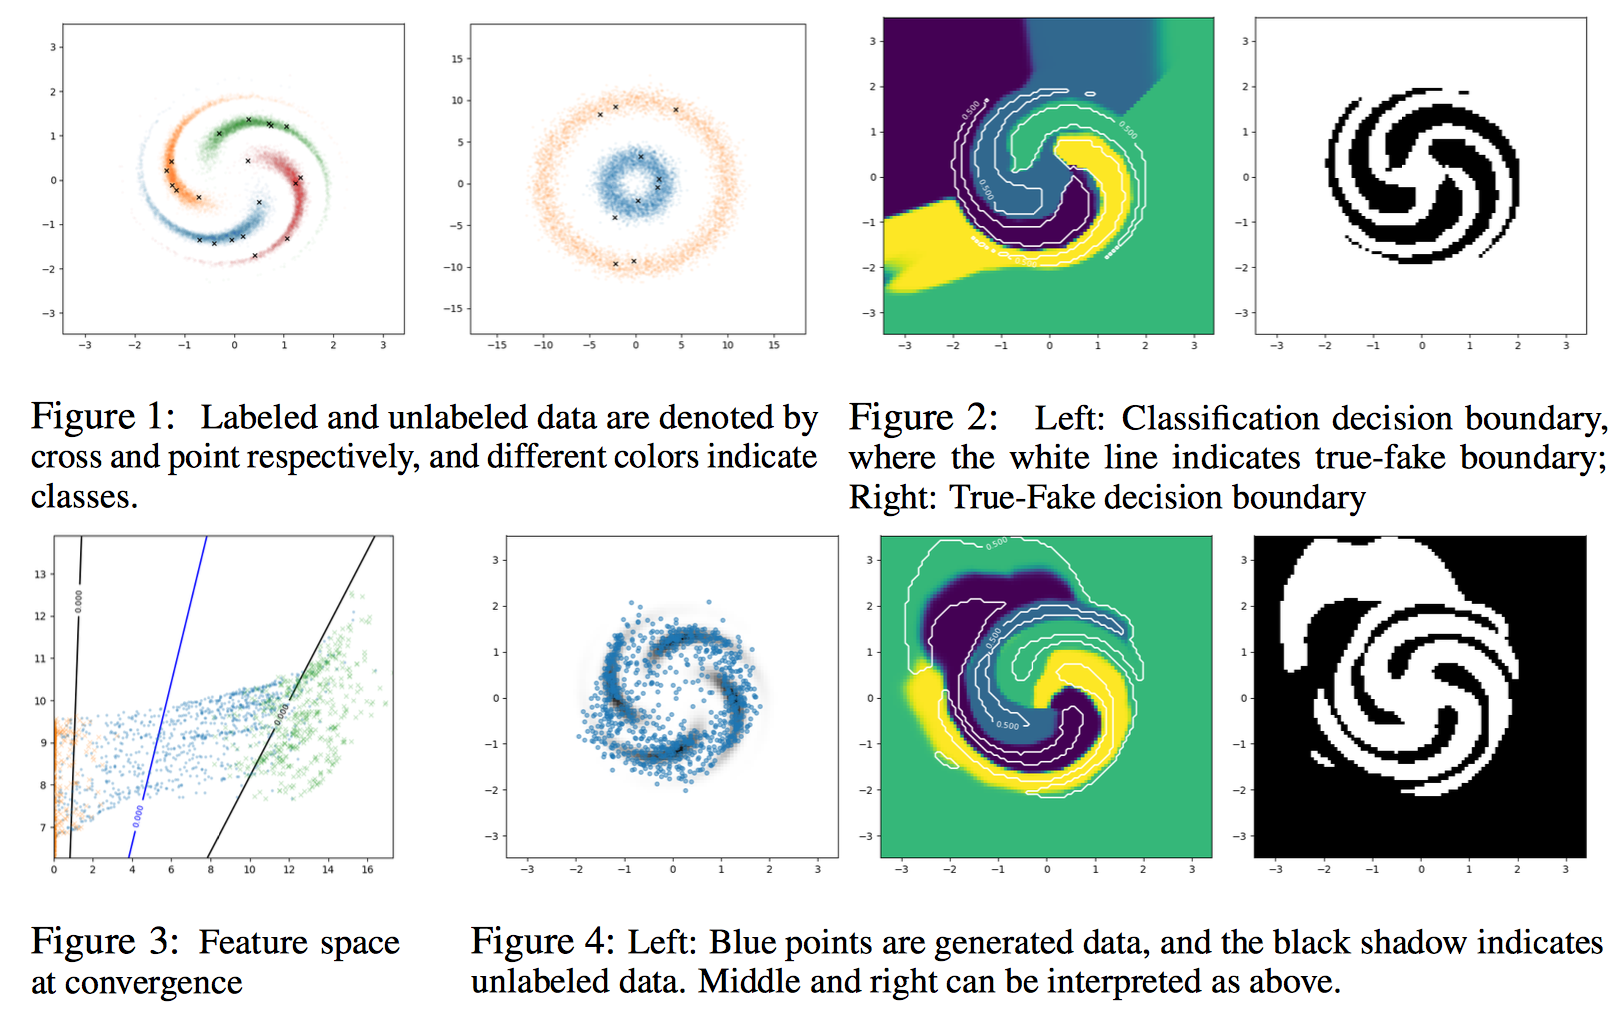
\includegraphics[width=\textwidth]{./img/33.png}
\caption{Semi-supervised GAN图解}
\label{fig:33}
\end{figure}
文章提出优化G的support的凸集内概率为$\frac{1}{Z}\frac{1}{p(x)}$这个分布的KL散度。但为了保证其他地方没有分布,否则KL散度没法算,还得加上原来的feature match使得生成的分布尽量靠近真实分布(又不能落在真实分布中)。\ref{fig:33}

最后G的loss是$$\min_G \quad -\mathcal{H}(p_G) + \mathbb{E}_{x \sim p_G} \log p(x) \mathbb{I}[p(x) > \epsilon]  + \|\mathbb{E}_{x \sim p_G} f(x) - \mathbb{E}_{x \sim \mathcal{U}} f(x)\|^2.
$$

第一项熵用类似与INFO GAN中的方法估计$-\mathcal{H}(p_G) \leq - \mathbb{E}_{x, z \sim p_G} \log q(z | x) = L_\text{VI}$,第二项用pixelCNN++\cite{DBLP:journals/corr/SalimansKCK17}的方法估计。
下面是判别器的损失函数,与之前类似,最后一项熵的意思是鼓励生成尖峰分布,使得判别出来的尽量靠近其中一个类。
\begin{equation}
\small
\begin{aligned}
\max_{D} \quad
& \mathbb{E}_{x, y \sim \mathcal{L}} \log p_D(y | x, y \leq K) + \mathbb{E}_{x \sim \mathcal{U}} \log p_D(y \leq K | x) + \\
& \mathbb{E}_{x \sim p_G} \log p_D(K + 1 | x)  + \mathbb{E}_{x \sim \mathcal{U}} \sum_{k = 1}^K p_D(k | x) \log p_D(k | x).
\label{eq:d_full}
\end{aligned}
\end{equation}
\bibliographystyle{plainnat}
\bibliography{sample}

\end{document}